\documentclass{article} % For LaTeX2e
\usepackage{nips15submit_e,times}
\usepackage{hyperref}
\usepackage{url}
\usepackage{graphicx}
\usepackage{float}
\usepackage{amsmath}
\usepackage{multirow,array}
\usepackage{listings}
\usepackage{amsfonts}
\usepackage{caption}
\usepackage{subfigure}
\usepackage{algorithm,algorithmic}
%\usepackage[UTF8]{ctex} uncomment if needs Chinese support
%\usepackage{fontspec}

%\documentstyle[nips14submit_09,times,art10]{article} % For LaTeX 2.09

\renewcommand{\algorithmicrequire}{ \textbf{Input:}} %Use Input in the format of Algorithm
\renewcommand{\algorithmicensure}{ \textbf{Output:}} %UseOutput in the format of Algorithm

\definecolor{mygreen}{rgb}{0,0.6,0}
\definecolor{mygray}{rgb}{0.5,0.5,0.5}
\definecolor{mymauve}{rgb}{0.58,0,0.82}
\lstset{ %
backgroundcolor=\color{white},   % choose the background color
basicstyle=\footnotesize\ttfamily,        % size of fonts used for the code
columns=fullflexible,
breaklines=true,                 % automatic line breaking only at whitespace
captionpos=b,                    % sets the caption-position to bottom
tabsize=4,
commentstyle=\color{mygreen},    % comment style
escapeinside={\%*}{*)},          % if you want to add LaTeX within your code
keywordstyle=\color{blue},       % keyword style
stringstyle=\color{mymauve}\ttfamily,     % string literal style
frame=single,
rulesepcolor=\color{red!20!green!20!blue!20},
% identifierstyle=\color{red},
language=python,
numbers=left
}

\title{Weekly Report(May 21 - May 27)}


\author{
Liu Junnan
}

% The \author macro works with any number of authors. There are two commands
% used to separate the names and addresses of multiple authors: \And and \AND.
%
% Using \And between authors leaves it to \LaTeX{} to determine where to break
% the lines. Using \AND forces a linebreak at that point. So, if \LaTeX{}
% puts 3 of 4 authors names on the first line, and the last on the second
% line, try using \AND instead of \And before the third author name.

\newcommand{\fix}{\marginpar{FIX}}
\newcommand{\new}{\marginpar{NEW}}

%\nipsfinalcopy % Uncomment for camera-ready version

\begin{document}


\maketitle

\begin{abstract}
This week I finished cs231n course and started to do assignment3.
\end{abstract}

\section{Work Done}
\subsection{RNN and LSTM}
\paragraph{RNN}
Unlike feedforward neural networks, recurrent neural networks take as their input not just the current input example they see, but also what they have perceived previously in time. The decision a recurrent net reached at time step $t-1$ affects the decision it will reach one moment later at time step $t$. So RNNs have two sources of input, the present and the recent past. The sequential information is preserved in the recurrent network’s hidden state, which manages to span many time steps as it cascades forward to affect the processing of each new example. One way to think about RNNs is this: they are a way to share weights over time. Therefore RNNs are good at processing sequences like image caption and machine translation. 

\begin{figure}[H]
	\centering
	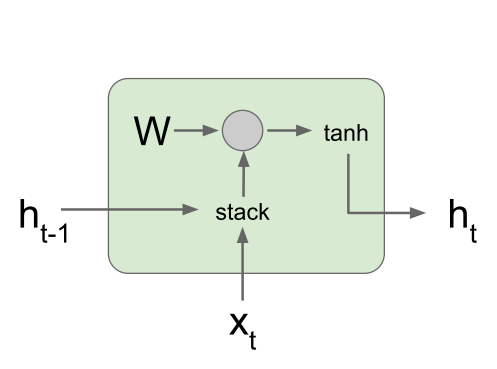
\includegraphics[width=.4\textwidth]{rnn.png}
	\caption{RNN unit}
\end{figure}

The forward pass of a RNN block can be mathematically described as:
$$h_t=f_W(h_{t-1},x_t)$$
where $h_t$ is the current hidden state at time step $t$; $f_W$ the function -- either sigmoid or tanh -- that squashes the sum of the weight input and hidden state,  making gradients workable for backpropagation; $h_{t_1}$ the previous hidden state; $x_t$ the input at the same time step.

Recurrent networks rely on an extension of backpropagation called backpropagation through time, or BPTT. Time, in this case, is simply expressed by a well-defined, ordered series of calculations linking one time step to the next, which is all backpropagation needs to work.

However, RNNs suffer a lot from vanishing/exploding gradient problems. Intuitively, backpropagation from $h_t$ to $h_{t-1}$ multiplies by $W_h$, so computing gradient of $h_0$ involves many factors of $W_h$. If the largest singular value of $W_h$ is greater than $1$, then exploding gradients would occur; on the contrary if the largest singular value of $W_h$ if less than $1$, then vanishing gradients would happen. Exploding gradients can be solved relatively easily, because they can be truncated or squashed. Vanishing gradients can become too small for computers to work with or for networks to learn – a harder problem to solve. 

\paragraph{LSTM}
Long short-term memory was proposed to solve vanishing gradient problem mentioned above. LSTMs design complicated cells that help preserve the error that can be backpropagated through time and layers.

\begin{figure}[H]
	\centering
	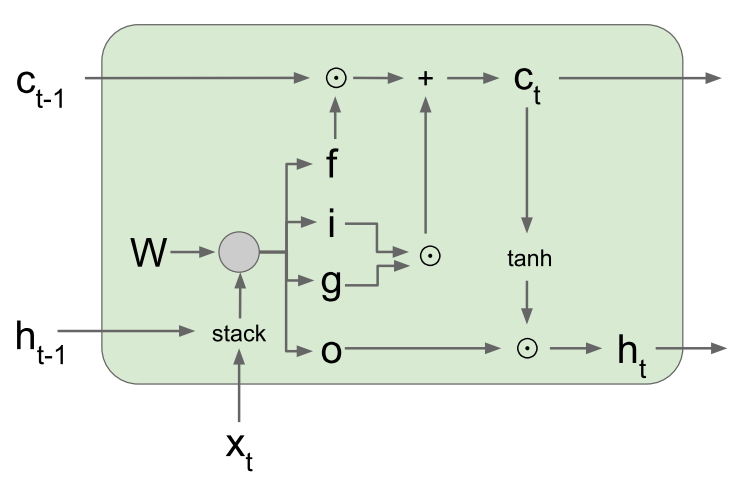
\includegraphics[width=.6\textwidth]{lstm.png}
	\caption{LSTM cell}
\end{figure}

The forward pass of a LSTM cell is defined as follows:
\begin{eqnarray}
\left(\begin{array}{c} i\\f\\o\\g \end{array}\right) &=& \left(\begin{array}{c} \sigma\\\sigma\\\sigma\\\tanh \end{array}\right) W \left(\begin{array}{c} h_{t_1}\\x_t \end{array}\right)  \label{eqn:lstm} \\
\nonumber c_t &=& f \odot c_{t_1} + i \odot g\\
\nonumber h_t &=& o \odot \tanh(c_t)

\end{eqnarray}
where $\odot$ is element-wise multiplication.

As described in equation(\ref{eqn:lstm})


\section{Plans}

\end{document}
